\documentclass[9pt,a4paper,twocolumn,twoside]{rho-class/rho}
\usepackage[english]{babel}

%----------------------------------------------------------
% Title
%----------------------------------------------------------

\doctype{Interim Report - INF398}
\title{3D Surface Anomaly Detection on MVTec 3D-AD: Classical Features vs. Deep Learning}

%----------------------------------------------------------
% Authors, Affiliations and dates
%----------------------------------------------------------

\author[{\textasteriskcentered},a,1]{Roman Oelfken, Jannike Andrea Hultengreen}

%----------------------------------------------------------
% Corresponding author-, Document- information
%----------------------------------------------------------

\journal{Introducción al aprendizaje automático}
\theday{\today}

%----------------------------------------------------------

\begin{document}

    \maketitle
    \thispagestyle{firststyle}

%----------------------------------------------------------
% Interim report sections
\section{Updated Problem and Objectives}

\subsection*{Updated problem statement}
This project investigates unsupervised industrial surface anomaly detection on the MVTec 3D-AD dataset \cite{bergmann2022mvtec3d}. The task is not formulated as standard supervised defect classification. Instead, models are trained only on defect-free samples and must assign high anomaly scores to abnormal test samples and, when possible, localize the affected regions. This setting follows the evaluation logic of MVTec 3D-AD and related industrial anomaly detection benchmarks \cite{bergmann2019mvtec,bergmann2022mvtec3d}.

The initial project plan compared explicit feature engineering against learned representations. During implementation, this formulation was refined. The first handcrafted baseline compressed each local patch into nine statistics, including mean height, standard deviation, gradient magnitude and roughness proxies. Qualitative inspection showed that this representation discarded too much spatial structure: small defects could become indistinguishable from sensor noise, and larger defects often required information beyond a single local descriptor. Therefore, the current classical baseline uses the raw normalized depth values of each patch, followed by PCA and a category-specific One-Class SVM \cite{scholkopf2001estimating}. This still remains a classical one-class model, but it is more directly comparable to the planned autoencoder because both methods operate on the same local depth-patch representation.

The current problem statement is thus more precise: we study how far local depth-only patch normality modeling can go on MVTec 3D-AD, and whether learned reconstruction models or additional RGB information are needed to capture defects that are not locally distinctive in geometry alone. This interim stage is especially useful because the first experiments already show that the choice of representation and context is as important as the choice of anomaly detector.

\subsection*{Updated objectives}

The primary objective is to implement and evaluate two unsupervised anomaly detection pipelines on MVTec 3D-AD under a unified experimental framework. The comparison focuses on predictive performance, localization quality, computational complexity and interpretability.

The updated research questions are:
\begin{itemize}
    \item How effective is a category-specific classical baseline based on raw normalized depth patches, PCA and One-Class SVM for 3D surface anomaly detection \cite{scholkopf2001estimating}?
    \item Does a compact deep learning model trained on normal samples learn more effective representations of surface regularity than local patch-based one-class methods \cite{li2025surveyindustrialad}?
    \item Does RGB information improve detection for defects that are weakly expressed in depth, such as contamination or color-related anomalies?
    \item What trade-offs emerge between predictive performance, localization quality, computational cost and interpretability when comparing classical, deep and multimodal variants?
\end{itemize}

\section{Proposed Solution}

\subsection*{Shared Patch-Based Pipeline}
Both approaches are built on the same preprocessing, patch extraction and scoring pipeline. Each raw XYZ sample is converted into a depth map by extracting the $Z$ channel. The object foreground is estimated from valid depth values, cropped with a margin, resized while preserving aspect ratio and snapped to the patch grid. The resulting processed map is normalized over object pixels only. This produces a consistent representation while avoiding distortions for elongated categories such as \textit{rope}.

The shared procedure is:
\begin{lstlisting}[basicstyle=\ttfamily\scriptsize,frame=single]
for each sample:
    load RGB and XYZ files
    extract depth = XYZ[..., 2]
    estimate foreground and crop object region
    resize depth and mask, preserving aspect ratio
    snap height/width to the patch grid
    normalize valid object depth values
    extract overlapping 32 x 32 patches
    score each patch with the selected model
    aggregate patch scores into an anomaly heatmap
    compute image score with top-k mean pooling
\end{lstlisting}

This design makes the comparison fair: classical and deep models see the same samples, the same processed coordinates, the same patch grid and the same image-level scoring rule. It also makes qualitative localization possible because patch scores can be aggregated back into image space.

\subsection*{Classical Baseline}
The current classical baseline is trained independently for each object category. Each valid $32 \times 32$ depth patch is converted into a vector of $1024$ normalized height values. Invalid or outside-object pixels are filled with the patch mean to avoid artificial border patterns. Features are standardized with a \texttt{StandardScaler}, reduced to $64$ components with PCA and modeled with an RBF One-Class SVM \cite{scholkopf2001estimating}. The model is trained only on normal training patches from the same category.

At inference time, every test image is decomposed into patches. The One-Class SVM decision scores are converted into anomaly scores, aggregated into a heatmap through overlap averaging and summarized into one image-level score using the mean of the top $5\%$ highest patch scores. Ground-truth masks are transformed with the same crop and resize geometry and drawn as contours on the qualitative figures.

\subsection*{Deep Learning Pipeline}
The planned deep baseline is a compact convolutional autoencoder trained on the same normal depth patches. Its input is initially a $1 \times 32 \times 32$ patch and its target is the reconstructed patch. The anomaly score will be the reconstruction residual, aggregated with the same overlap-aware mechanism used by the classical model. This provides a controlled comparison between a one-class boundary in PCA feature space and a learned reconstruction model over the same local representation.

\subsection*{RGB and Multimodal Extension}
Because early results indicate that some defects are weak in depth but visible in color, the final plan includes a controlled modality ablation. The intended variants are depth only, RGB only and depth+RGB. RGB images will be cropped and resized with the same geometry as the depth maps, but they will not be normalized per image with min-max scaling, since that could remove color-based anomaly information. This extension is planned as an adjustment motivated by the interim results rather than as an unrelated add-on.

\section{Implementation Plan}
The implementation is organized into data preparation, patch extraction, model training, inference and evaluation. Table~\ref{tab:implementation-status} summarizes what has been completed at the interim stage and what remains for the final submission.

\begin{table}[H]
\centering
\scriptsize
\renewcommand{\arraystretch}{1.25}

\caption{Implementation status at the interim submission.}

\begin{tabularx}{\columnwidth}{|
>{\raggedright\arraybackslash}p{1.8cm}|
>{\raggedright\arraybackslash}p{2cm}|
X|
>{\centering\arraybackslash}p{1.4cm}|}

\hline


\textbf{Module} &
\textbf{Component} &
\textbf{Functionality} &
\textbf{Status} \\ \hline

Data Preprocessing &
Dataset Indexing &
Parse MVTec 3D-AD structure, splits and metadata &
\cellcolor{implgreen}Implemented \\ \cline{2-4}

&
Depth Preprocessing &
Extract depth channel, mask invalid values, crop, resize and normalize depth maps &
\cellcolor{implgreen}Implemented \\ \hline

Patch Extraction &
Patch Generation &
Generate overlapping $32 \times 32$ patches &
\cellcolor{implgreen}Implemented \\ \cline{2-4}

&
Score Aggregation &
Aggregate patch scores into image space &
\cellcolor{implgreen}Implemented \\ \hline

Classical Baseline &
Current Baseline &
Use raw depth patches with PCA and One-Class SVM &
\cellcolor{implgreen}Implemented \\ \cline{2-4}

&
Test Inference &
Generate image scores and anomaly maps &
\cellcolor{implgreen}Implemented \\ \cline{2-4}

&
Preliminary RGB Analysis &
Analyze whether RGB contains useful anomaly information &
\cellcolor{implgreen}Implemented \\ \cline{2-4}

&
Future Extensions &
Explore RGB-enhanced or multimodal representations &
\cellcolor{planblue}Planned \\ \hline

Deep Learning Model &
Autoencoder Design &
Design convolutional autoencoder &
\cellcolor{progYellow}In Progress \\ \cline{2-4}

&
Autoencoder Training &
Train reconstruction-based model &
\cellcolor{planblue}Planned \\ \hline

Evaluation \& Visualization &
Classical Evaluation &
Compute AUROC and AP for the classical baseline &
\cellcolor{implgreen}Implemented \\ \cline{2-4}

&
Classical Heatmaps &
Generate anomaly heatmaps for the classical baseline &
\cellcolor{implgreen}Implemented \\ \cline{2-4}

&
Autoencoder Evaluation &
Compute AUROC, AP and heatmaps for the autoencoder &
\cellcolor{planblue}Planned \\ \cline{2-4}

&
Comparative Evaluation &
Compare classical and deep learning results &
\cellcolor{planblue}Planned \\ \hline

\end{tabularx}

\label{tab:implementation-status}
\end{table}

\subsection*{Repository organization and reproducibility}
The implementation is organized as a reproducible repository rather than as isolated scripts. Shared parameters are stored in \texttt{configs/}, reusable code lives in \texttt{src/}, runnable entry points are placed in \texttt{scripts/}, visual evidence is saved in \texttt{fig/}, and trained models, logs and metrics are stored under \texttt{outputs/}. The main modules are separated by responsibility: \texttt{src/data/} handles indexing, preprocessing and patch extraction; \texttt{src/features/} contains feature construction; \texttt{src/models/} contains anomaly models; \texttt{src/training/} and \texttt{src/inference/} implement model execution; and \texttt{src/evaluation/} contains metrics and visualization utilities.

The current pipeline can be reproduced through documented commands:
\begin{lstlisting}[basicstyle=\ttfamily\scriptsize,frame=single]
conda env create -f environment.yml
conda activate mvtec-3d-ad
pip install -e .
python scripts/prepare_data.py
python scripts/train_classical.py
python scripts/infer_classical.py --split test
python -m unittest discover tests
\end{lstlisting}

This structure makes the interim results auditable: the reported metrics come from saved CSV files, the heatmaps are generated by the inference pipeline, and the classical models are stored per category with their scaler, PCA transform and feature metadata. The next implementation priority is to complete the autoencoder training/inference path and run a controlled modality ablation before the final comparison.

\section{Dataset and Preprocessing}

\subsection*{Dataset}
We use the MVTec 3D-AD dataset, a benchmark designed for unsupervised 3D anomaly detection and localization \cite{bergmann2022mvtec3d}. The dataset is publicly available from the MVTec research page.\footnote{\url{https://www.mvtec.com/company/research/datasets/mvtec-3d-ad}} The current pipeline indexes all ten categories available in the local release: bagel, cable gland, carrot, cookie, dowel, foam, peach, potato, rope and tire.

The indexed data contain $4147$ samples in total. The training split contains $2656$ normal samples, the validation split contains $294$ normal samples and the test split contains $1197$ samples, of which $249$ are normal and $948$ are anomalous. Training and validation therefore preserve the unsupervised setting: no defective samples are used to fit the normality models.

\begin{figure*}[t]
    \centering
    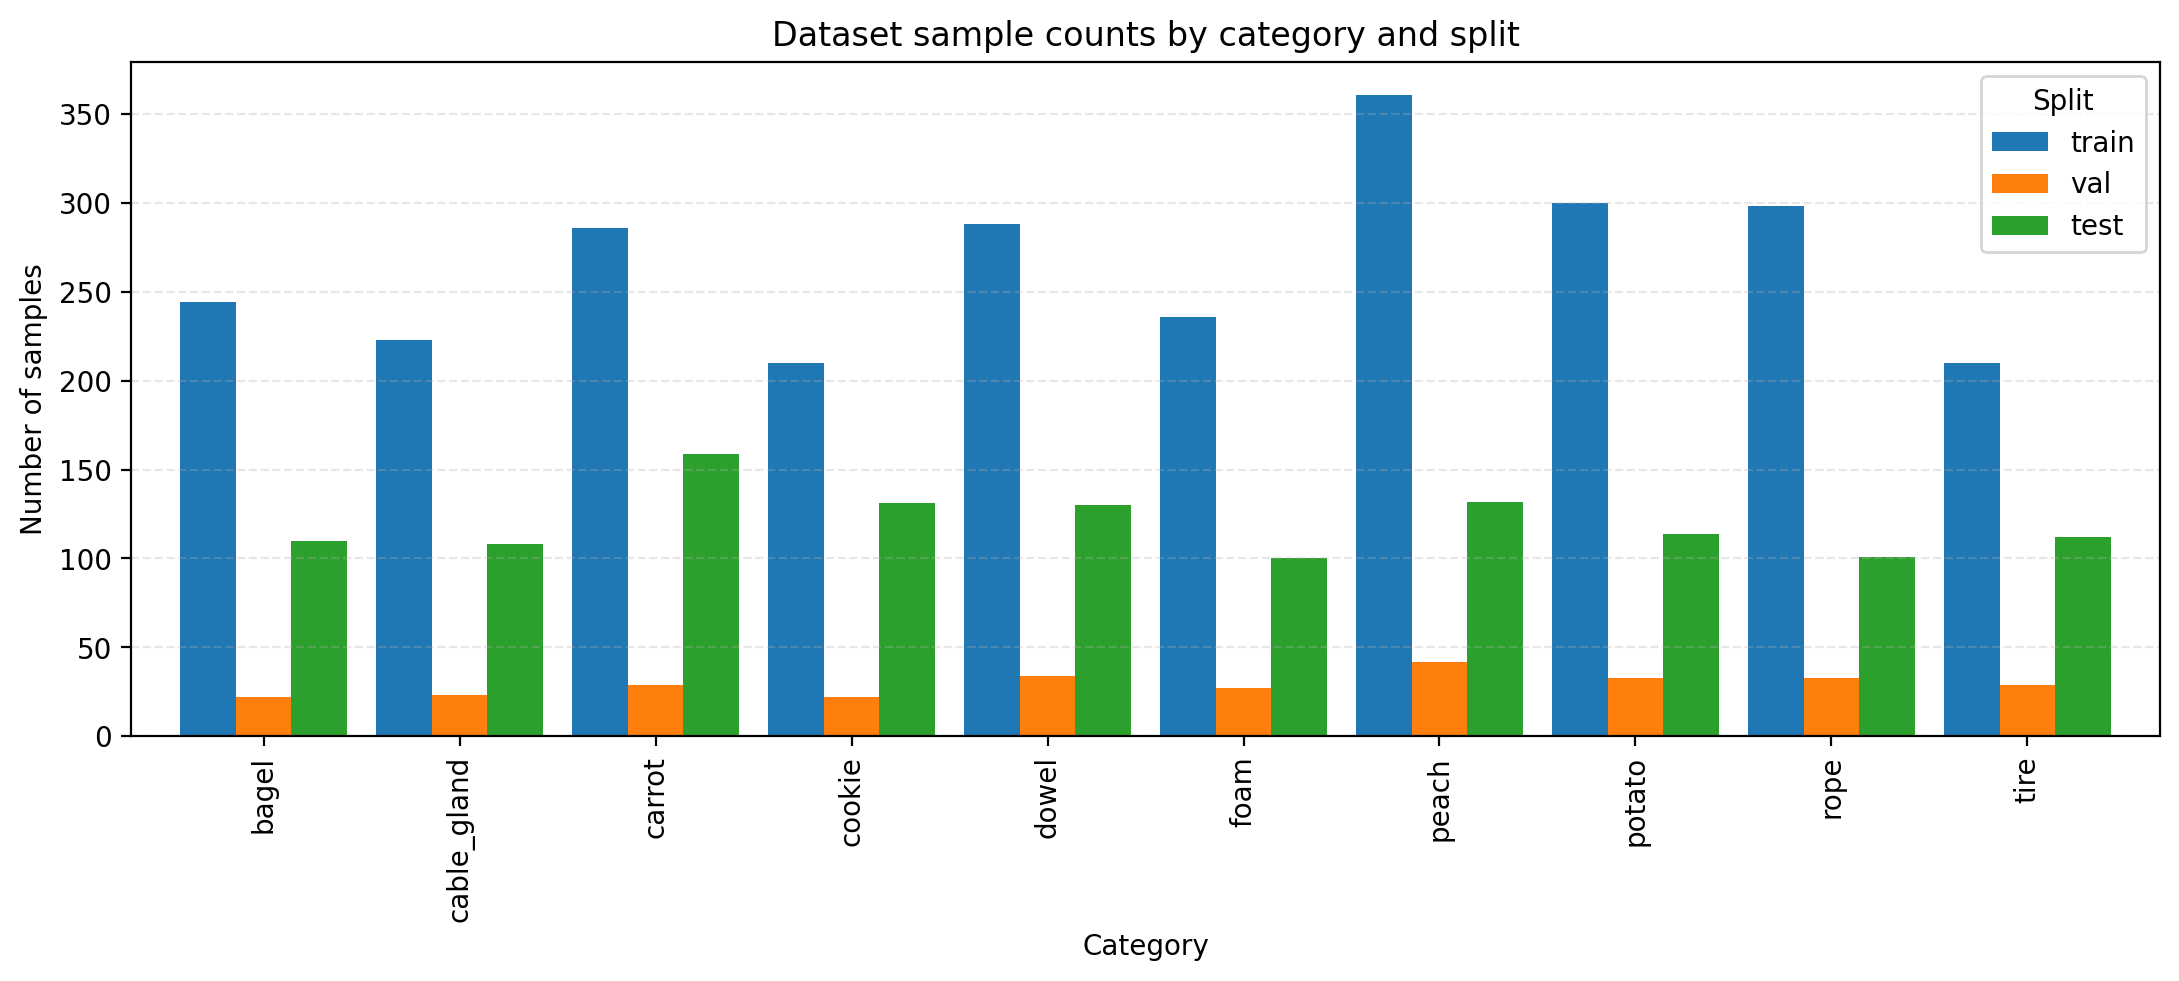
\includegraphics[width=0.92\textwidth]{figures/index_summary.png}
    \caption{Indexed MVTec 3D-AD samples by category, split and label.}
    \label{fig:index-summary}
\end{figure*}

\subsection*{Depth preprocessing}
The MVTec 3D-AD samples provide RGB images, XYZ point maps and ground-truth masks for defective test samples. The current shared representation is a depth map derived from the $Z$ channel of the raw XYZ file. Preprocessing performs valid-depth masking, foreground estimation, object cropping with a configurable margin, aspect-preserving resize, patch-grid snapping and per-image normalization over object pixels only. The processed output stores both the normalized depth map and a foreground mask.

The aspect-preserving resize is important because forcing all objects into a square canvas can introduce large empty areas and distort the patch raster. This was especially visible for elongated categories such as \textit{rope}. The final processed dimensions are snapped so that fixed-size patches land cleanly on image borders.

\begin{figure}[H]
    \centering
    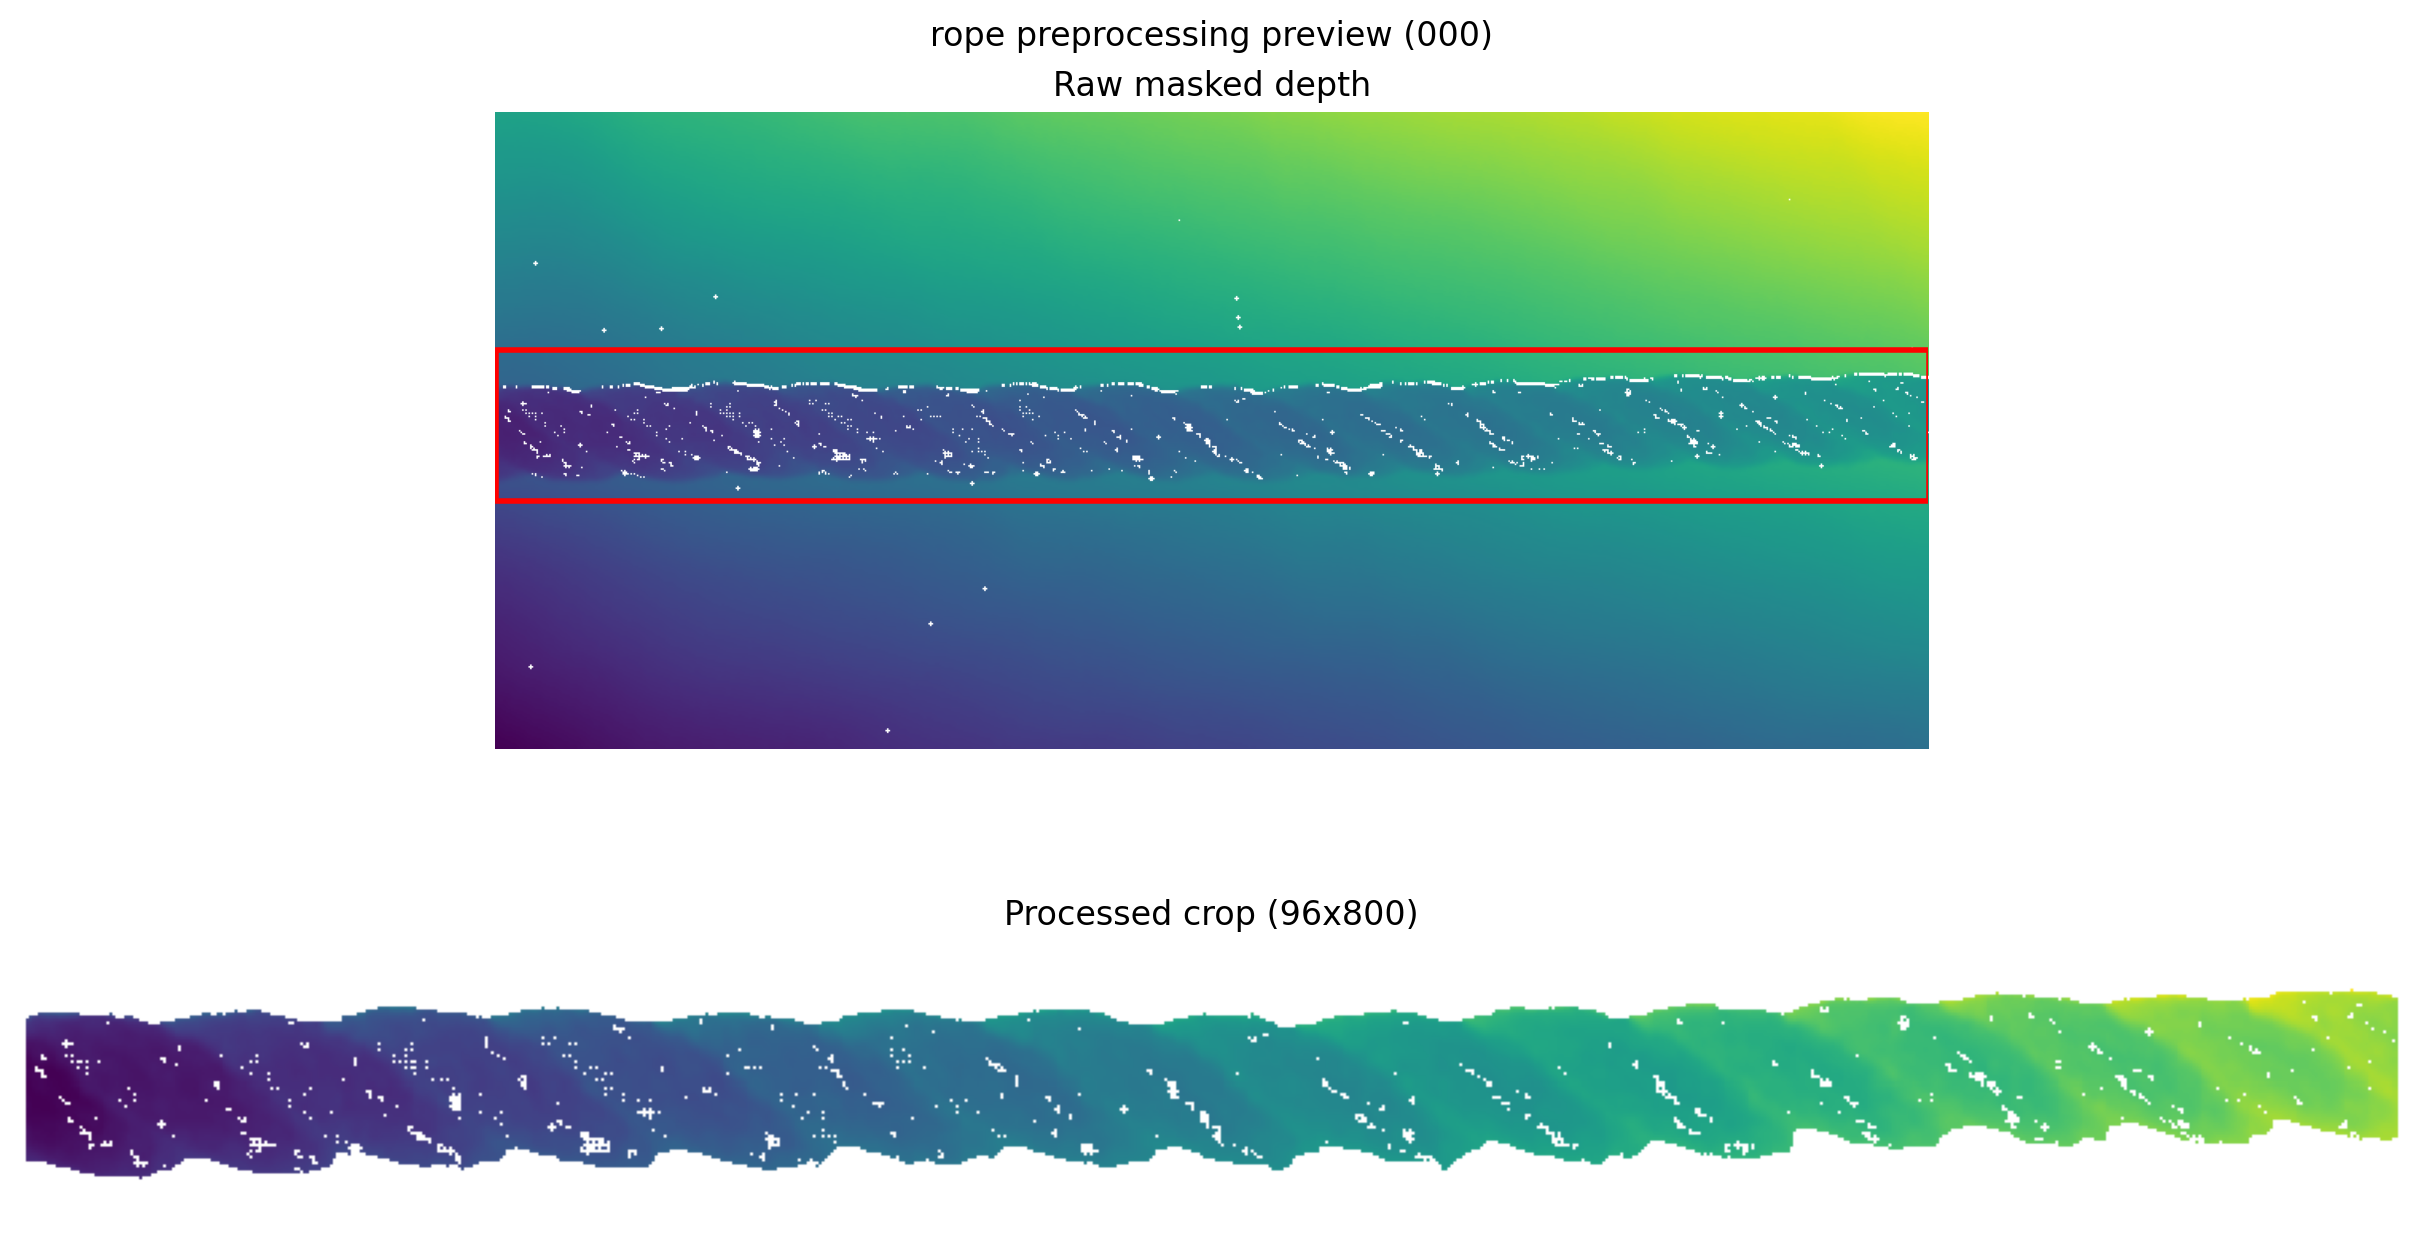
\includegraphics[width=\columnwidth]{figures/rope_raw_vs_processed.png}
    \caption{Example of the raw-to-processed depth transformation for an elongated object.}
    \label{fig:preprocessing-rope}
\end{figure}

\subsection*{Patch Extraction}
After preprocessing, each normalized depth map is divided into overlapping $32 \times 32$ local patches with stride $16 \times 16$. Patch coordinates are generated deterministically in row-major order. During training, patches with too little valid object area are skipped. During inference, patch scores are aggregated back to image space by averaging overlapping contributions. This patch-based representation increases the number of normal training examples and provides a direct route from local scores to anomaly heatmaps.

\section{Preliminary Experiments}

\subsection*{Classical baseline setup}
The first implemented experiment evaluates the category-specific One-Class SVM baseline on normalized depth patches. The final feature path is:
\[
32 \times 32 \text{ depth patch}
\rightarrow 1024 \text{ values}
\rightarrow \text{StandardScaler}
\rightarrow \text{PCA}(64)
\rightarrow \text{One-Class SVM}.
\]
Each category has its own scaler, PCA transform and model. The training run used $200000$ normal training patches and $47913$ validation patches across the ten categories. Test inference evaluated $1197$ images and scored $238113$ patches.

\subsection*{Image-level results}
The current depth-only classical baseline is informative but not yet strong enough for the final target. Overall image-level performance on the test split is shown in Table~\ref{tab:classical-results}. AUROC is the main ranking metric, while AP is reported because precision-recall measures are common in anomaly detection. AP should be interpreted together with AUROC because the test split contains more anomalous than normal samples.

\begin{table}[H]
\centering
\caption{Image-level performance of the current classical baseline.}
\label{tab:classical-results}
\begin{tabular}{lc}
\toprule
\textbf{Metric} & \textbf{Value} \\
\midrule
Overall AUROC & 0.5517 \\
Overall AP & 0.8293 \\
Macro AUROC & 0.5415 \\
Macro AP & 0.8307 \\
\bottomrule
\end{tabular}
\end{table}

Performance varies strongly by category. The best category is \textit{rope} with AUROC $0.8071$, followed by \textit{cookie} with $0.6969$ and \textit{peach} with $0.6705$. Several categories remain close to or below random ranking, including \textit{tire} ($0.4221$), \textit{dowel} ($0.4301$), \textit{foam} ($0.4350$) and \textit{bagel} ($0.4597$). This pattern suggests that local depth information is useful for some object-defect combinations, but insufficient for others.

\begin{table}[H]
\centering
\scriptsize
\caption{Per-category AUROC for the current depth-only classical baseline.}
\label{tab:category-auroc}
\begin{tabular}{lclc}
\toprule
\textbf{Category} & \textbf{AUROC} & \textbf{Category} & \textbf{AUROC} \\
\midrule
rope & 0.8071 & carrot & 0.5017 \\
cookie & 0.6969 & potato & 0.4773 \\
peach & 0.6705 & bagel & 0.4597 \\
cable gland & 0.5145 & foam & 0.4350 \\
dowel & 0.4301 & tire & 0.4221 \\
\bottomrule
\end{tabular}
\end{table}

\subsection*{Qualitative localization}
The classical model also produces anomaly heatmaps by aggregating patch scores. Ground-truth masks are transformed into the processed coordinate system and drawn as cyan contours. Figure~\ref{fig:rope-heatmap} should be read from left to right: the first panel shows the processed depth map used by the model, the second panel shows the display-normalized anomaly heatmap, and the third panel overlays the heatmap on the depth image. Brighter colors in the heatmap indicate higher local anomaly scores; they are useful for qualitative localization, but they are not calibrated probabilities.

The example shows a case where the local depth baseline captures useful signal, because high-score regions overlap part of the annotated defect contour. At the same time, responses outside the contour illustrate the main limitation of the current model: local patch scores can be noisy when the defect is subtle or when normal geometric variation resembles an anomaly. In other categories, this effect is stronger and motivates the planned autoencoder and RGB/multimodal experiments.

\begin{figure}[H]
    \centering
    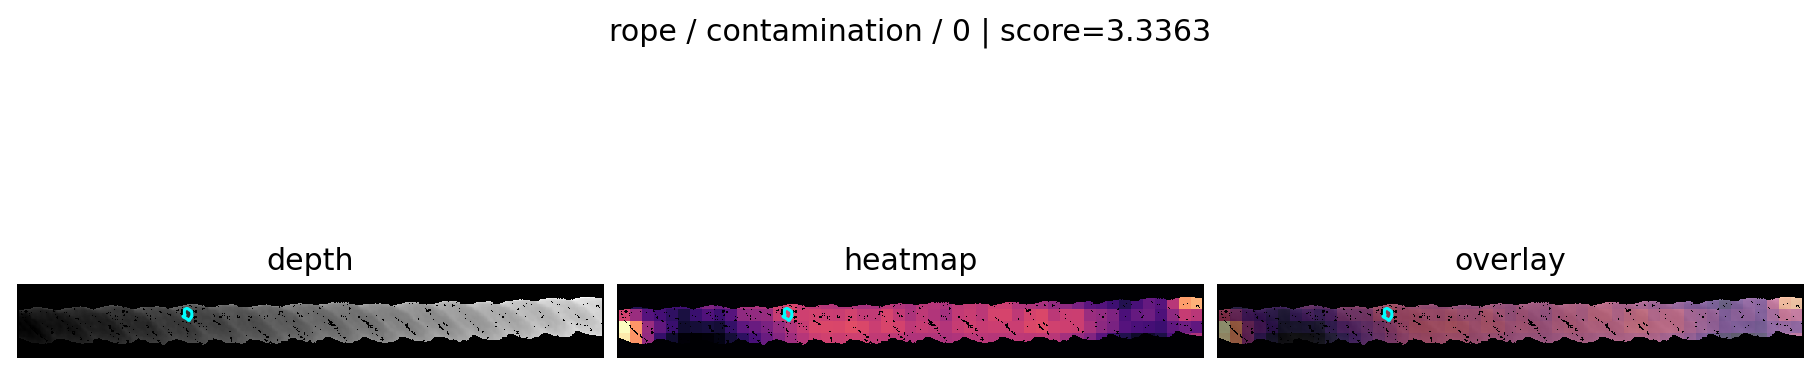
\includegraphics[width=\columnwidth]{figures/rope_contamination_heatmap.png}
    \caption{Qualitative output for a rope contamination sample. Left: processed depth map. Middle: normalized anomaly heatmap from aggregated One-Class SVM patch scores. Right: heatmap overlaid on depth. Cyan contours show the transformed ground-truth defect mask.}
    \label{fig:rope-heatmap}
\end{figure}

\subsection*{RGB investigation}
Because some defects are difficult to distinguish in depth alone, we performed a preliminary RGB signal check. RGB files are present for all $1197$ test samples, and their sizes match the ground-truth masks. This means RGB can be transformed using the same crop and resize geometry as the depth maps.

The signal check compared RGB values inside the ground-truth defect region with a local surrounding context ring. It is not a trained model, but it estimates whether color provides useful anomaly information. The strongest median RGB signal was observed for \textit{cookie} ($1.965$), \textit{potato} ($1.163$), \textit{peach} ($1.145$) and \textit{foam} ($0.998$). Particularly strong defect-type signals appeared for cookie contamination ($5.419$), cookie hole ($3.116$), potato contamination ($2.379$) and peach contamination ($2.265$). Weak signals were found for some structural or subtle cases, such as tire combined defects ($0.315$) and cable gland holes ($0.491$).

This supports a concrete adjustment to the final plan: RGB should be tested as an additional modality, especially for contamination and color-related defects, but it should not replace depth because many anomalies remain geometric or contextual.

\section{Risks and Adjustments}

\subsection*{Risks identified so far}
The main technical risk is that many defects are not locally distinctive in depth alone. Some anomalous patches look plausible when viewed without broader object context, while some larger structural defects require global shape, position or neighborhood information. This explains why the local One-Class SVM baseline works reasonably for some categories but fails to separate normal and anomalous samples reliably overall.

The second risk is representation quality. The original handcrafted descriptors were interpretable but too compressed. Replacing them with raw depth patches improved methodological fairness with the planned autoencoder, but the current AUROC still shows that model capacity alone may not solve missing-context defects.

The third risk is time and implementation complexity. Completing the autoencoder, adding RGB preprocessing and running modality ablations must be done without destabilizing the already working shared pipeline.

\subsection*{Plan adjustments for the final submission}
Based on the interim results, the plan has been adjusted in four ways. First, the classical baseline is now defined as raw normalized depth patches plus PCA and One-Class SVM, while the nine-statistic handcrafted representation is kept only as an early weak baseline. Second, the autoencoder will use exactly the same patch extraction, split and scoring logic, so the comparison remains controlled. Third, RGB preprocessing will be added with the same crop and resize geometry as depth, followed by a modality ablation comparing depth, RGB and depth+RGB. Fourth, if both classical and autoencoder approaches remain weak, the final analysis will explicitly discuss context limitations and consider larger patches, multi-scale patches or position-aware features as future extensions.

These adjustments keep the project within scope while making the final comparison more meaningful. The interim result is therefore not only a partial implementation milestone, but also evidence that the project direction should shift from "which model is better?" toward the more precise question "which representation and context are sufficient for each type of 3D anomaly?"

\section*{Repository}
\addcontentsline{toc}{section}{Repository}

The source code, configuration files, generated metrics and visual outputs are maintained in the project repository.

\begin{center}
    \setlength{\tabcolsep}{3pt}
    \begin{tabular}{cl}
         \faGithub &
         \href{https://github.com/romanoen/Explainable-Surface-Defect-Detection-on-MVTec-AD-INF398}{Github - Surface defect detection on MVTec AD -INF398 }\\
    \end{tabular}
\end{center}
\printbibliography[title={Updated Bibliography}]

%----------------------------------------------------------

\end{document}
